\documentclass[a4paper,14pt]{article}

\usepackage{comment} % Para comentar várias linhas ao mesmo tempo

%matemática
\usepackage{amsmath}
\usepackage{amssymb}

%diagramação
\usepackage{extsizes}
\everymath{\displaystyle}
\usepackage{geometry}
\usepackage{fancyhdr}
\usepackage{multicol}
\usepackage{graphicx}
\usepackage[brazil]{babel}
\usepackage[shortlabels]{enumitem}
\usepackage{cancel}
\usepackage{textcomp}
\usepackage{tcolorbox}

%tabelas
\usepackage{array} % Para melhor formatação de tabelas
\usepackage{longtable}
\usepackage{booktabs}  % Para linhas horizontais mais bonitas
\usepackage{float}   % Para usar o modificador [H]
\usepackage{caption} % Para usar legendas em tabelas
\usepackage{wrapfig} % Para usar tabelas e figuras flutuantes
\usepackage{xcolor} % Para cores do fundo de tabelas
\usepackage{colortbl} % Para cores do fundo de tabelas
\usepackage{upgreek} % Para inserir caracteres gregos

%tikzpicture
\begin{comment}
	\usepackage{tikz}
	\usepackage{scalerel}
	\usepackage{pict2e}
	\usepackage{tkz-euclide}
	\usetikzlibrary{calc}
	\usetikzlibrary{patterns,arrows.meta}
	\usetikzlibrary{shadows}
	\usetikzlibrary{external}
\end{comment}


%pgfplots
\usepackage{pgfplots}
\pgfplotsset{compat=newest}
\usepgfplotslibrary{statistics}
\usepgfplotslibrary{fillbetween}

%colours
\usepackage{xcolor}



\columnsep=2cm
\hoffset=0cm
\textwidth=8cm
\setlength{\columnseprule}{.1pt}
\setlength{\columnsep}{2cm}
\renewcommand{\headrulewidth}{0pt}
\geometry{top=1in, bottom=1in, left=0.7in, right=0.5in}

\pagestyle{fancy}
\fancyhf{}
\fancyfoot[C]{\thepage}

\begin{document}
	
	\noindent\textbf{6FMA156 - Matemática} 
	
	\begin{center}Revisão de números inteiros (Versão estudante)
	\end{center}
	
	\noindent\textbf{Nome:} \underline{\hspace{10cm}}
	\noindent\textbf{Data:} \underline{\hspace{4cm}}
	
	%\section*{Questões de Matemática}
	
	\begin{multicols}{2}
	    \noindent \begin{itemize}
	    	\item \textbf{Representação na reta} \\
	    	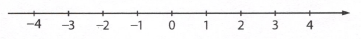
\includegraphics[width=1\linewidth]{6FMA156_imagens/imagem1}
	    	\item \textbf{Oposto ou simétrico}
	    	\begin{itemize}[label=\scriptsize$\blacksquare$]
	    		\item O oposto de 2 é -2.
	    		\item O oposto de -5 é -(-5) = 5.
	    	\end{itemize}
	    	\item \textbf{Módulo ou valor absoluto}
	    	\[|x| = 
	    	\begin{cases} 
	    		x, \text{se } x \geq 0 \\ 
	    		-x, \text{se } x < 0 
	    	\end{cases}\]
	    	\item \textbf{Multiplicação ou divisão}
	    	\begin{itemize}[label=\scriptsize$\blacksquare$]
	    		\item Positivo com positivo é positivo.
	    		\item Positivo com negativo é negativo.
	    		\item Negativo com positivo é negativo.
	    		\item Negativo com negativo é positivo.
	    	\end{itemize}
	    	\item \textbf{Potenciação}
	    	\begin{itemize}[label=\scriptsize$\blacksquare$]
	    		\item $a^m \cdot a^n = a^{m + n}$
	    		\item $\frac{a^m}{a^n} = a^{m - n}$
	    		\item $a^m \cdot b^m = (a \cdot b)^m$
	    		\item $(a^m)^n = a^{m \cdot n}$
	    		\item $a^{m^{n}} = a^{(m^n)}$
	    		\item $a^{-n} = \frac{1}{a^n}$
	    	\end{itemize}
	    \end{itemize} 
		\noindent\textsubscript{--------------------------------------------------------------------------}
		\begin{enumerate} 
			\item Determine o que se pede:
			\begin{enumerate}[a)]
				\item O oposto de -4. \\\\\\\\\\\\
				\item O simétrico do oposto de -10. \\\\\\\\\\\\
				\item O módulo do simétrico de 7. \\\\\\\\\\\\
				\item O oposto do módulo do simétrico de 3. \newpage
			\end{enumerate}
			\item Aplique as propriedades e reduza a uma única potência:
			\begin{enumerate}[a)]
				\item $\frac{2^{12} \cdot 2^7}{2^8}$ \\\\\\\\\\\\\\\\\\\\\\\\\\\\\\\\\\\\
				\item $\frac{\bigg[4^{13} : 4^5\bigg]^{-3}}{4^{-20}}$ \\\\\\\\\\\\\\\\\\\\\\\\\\\\\\\\
				\item $\frac{512 \cdot 64}{2 048}$ \\\\\\\\\\\\\\\\\\\\\\\\\\\\\\\\\\\\
				\item $\frac{[25 \cdot 125]^3}{(625)^4}$ \newpage
			\end{enumerate}
			\item Resolva as expressões:
			\begin{enumerate}[a)]
				\item $\bigg[5 - 3(7 - 13) + (-4)^2\bigg]$ \\\\\\\\\\\\\\\\\\\\\\\\\\\\\\\\\\\\\\\\\\\\\\\\\\\\\\\\\\\\\\\\\\\\\\\\
				\scriptsize\item $\bigg\{\bigg[(-9) \cdot (-6) + 2 \cdot(-4)^3 + 3 \cdot (-2)^5\bigg] + (-3 - 4)\bigg\}$ \\\\\\\\\\\\\\\\\\\\\\\\\\\\\\\\\\\\\\\\\\\\\\\\\\\\\\\\\\\\
			\end{enumerate}
			%51 a 53
			\normalsize \item Utilize as propriedades e reduza as expressões a uma única potência:
			\begin{enumerate}[a)]
				\item $\frac{\bigg[1 024 \cdot (16)^{-3}\bigg]^4}{\bigg[256 \cdot 4^{2^{3}}\bigg]^3}$ \\\\\\\\\\\\\\\\\\\\\\\\\\\\\\\\
				\item $\frac{\bigg(2187 \cdot 9^{2^{2}}\bigg)^{-3}}{243^{-2} \cdot 27^5}$ \newpage
			\end{enumerate}
			\item Resolva as expressões:
			\begin{enumerate}[a)]
				\item $\{[4 \cdot (-5) + 3^3 - 2] + 5\} \cdot 7$ \\\\\\\\\\\\\\\\\\\\\\\\\\\\\\\\\\\\\\\\
				\item $[2 - |-2| + 7 + (-3)] - 4$ \\\\\\\\\\\\\\\\\\\\\\\\\\\\\\\\
			\end{enumerate}
			\item Resolva as expressões:
			\begin{enumerate}[a)]
				\item $[4^3 \cdot 4^{-2} + (2^5 + 2 - 3^4 \cdot 3^{-3})] - 5^2$  \\\\\\\\\\\\\\\\\\\\\\\\\\\\\\\\\\\\\\\\\\
				\small\item $\bigg\{\frac{1}{4} + 0,\overline{6} - \bigg[5\frac{1}{3} - 6\frac{3}{5}(0,\overline{42} + 0,\overline{54})\bigg]\bigg\}$ \newpage
				\normalsize\item $\dfrac{\dfrac{4^3}{4} - \dfrac{3^4}{3}}{[7 \cdot (-1)^8 + 5^0]}$ \\\\\\\\\\\\\\\\\\\\
			\end{enumerate}
		\end{enumerate}
		$~$ \\ $~$ \\ $~$ \\ $~$ \\ $~$ \\ $~$ \\ $~$ \\ $~$ \\ $~$ \\ $~$ \\ $~$ \\ $~$ \\ $~$ \\ $~$ \\ $~$ \\ $~$ \\ $~$ \\ $~$ \\ $~$ \\ $~$ \\ $~$ \\ $~$ \\ $~$ \\ $~$ \\ $~$ \\ $~$ \\ $~$ \\ $~$ \\ $~$ \\ $~$ \\ $~$ \\ $~$ \\ $~$ \\ $~$ \\ $~$ \\ $~$ \\ $~$ \\ $~$ \\ $~$ \\ $~$ \\ $~$ \\ $~$ \\ $~$ \\ $~$ \\ $~$ \\ $~$ \\ $~$ \\ $~$ \\ $~$ \\ $~$ \\ $~$ \\ $~$ \\ $~$ \\ $~$ \\ $~$ \\ $~$ \\ $~$ \\ $~$ \\ $~$ \\ $~$ \\ $~$ \\ $~$ \\ $~$ \\ $~$ \\ $~$ \\ $~$ \\ $~$ \\ $~$ \\ $~$ \\ $~$ \\ $~$ 
	\end{multicols}
\end{document}